\documentclass[a4paper, 12pt]{article}
\usepackage{graphicx}
\usepackage[margin=2cm]{geometry}
\usepackage[hidelinks]{hyperref}
\usepackage[croatian]{babel}
\usepackage[sorting=none]{biblatex}
    \addbibresource{ref.bib}
\usepackage{float}


% Boje za kod:
\usepackage{xcolor,graphicx}
\usepackage{listings}
\usepackage{amsmath}

\definecolor{solarized-base03}{RGB}{0, 43, 54}
\definecolor{solarized-base02}{RGB}{7, 54, 66}
\definecolor{solarized-base01}{RGB}{88, 110, 117}
\definecolor{solarized-base00}{RGB}{101, 123, 131}
\definecolor{solarized-base0}{RGB}{131, 148, 150}
\definecolor{solarized-base1}{RGB}{147, 161, 161}
\definecolor{solarized-base2}{RGB}{238, 232, 213}
\definecolor{solarized-base3}{RGB}{253, 246, 227}
\definecolor{solarized-yellow}{RGB}{181, 137, 0}
\definecolor{solarized-orange}{RGB}{203, 75, 22}
\definecolor{solarized-red}{RGB}{220, 50, 47}
\definecolor{solarized-magenta}{RGB}{211, 54, 130}
\definecolor{solarized-violet}{RGB}{108, 113, 196}
\definecolor{solarized-blue}{RGB}{38, 139, 210}
\definecolor{solarized-cyan}{RGB}{42, 161, 198}
\definecolor{solarized-green}{RGB}{133, 153, 0}

\lstset{
  basicstyle=\footnotesize\ttfamily\color{solarized-base00},
  keywordstyle=\color{solarized-blue}\bfseries,
  commentstyle=\color{solarized-base1},
  stringstyle=\color{solarized-cyan},
  identifierstyle=\color{solarized-violet},
  numberstyle=\tiny\color{solarized-base01},
  numbers=left,
  firstnumber=1,
  stepnumber=1,
  showstringspaces=false,
  tabsize=4,
  frame=none,
  framerule=1pt,
  framexleftmargin=5pt,
  framexrightmargin=5pt,
  framextopmargin=3pt,
  framexbottommargin=3pt,
  backgroundcolor=\color{solarized-base3},
  rulecolor=\color{solarized-base01},
  breaklines=true,
  breakatwhitespace=true,
  language=C++
}


\begin{document}
\noindent
Univerzitet u Sarajevu\\
Elektrotehnički fakultet\\
Predmet: Uvod u digitalnu obradu slike\\
Predmetni profesor: prof. dr Emir Sokić\\
Autor: Berina Biberović\\
Akademska godina: 2022/2023.


\begin{center}
    \section*{Tutorijal 3}
    \subsection*{Operacije nad slikom u prostornom domenu}
\end{center}

\subsection*{Procesiranje slike u prostornom domenu}

Procesiranje monohromatske slike u prostornom domenu predstavlja primjenu operatora $T$ nad datom slikom $f(x, y)$ u domenu $(x, y)$ kako bi se dobila rezultantna slika $g(x, y)$. Možemo razlikovati dva tipa procesiranja slike u prostornom domenu - transformacija vrijednosti i transformacija korištenjem maske.

\subsubsection*{Transformacija vrijednosti}

Transformacija vrijednosti (ili drugim imenom mapiranje intenziteta) podrazumijeva da operator za izračunavanje vrijednosti zahtjeva okolinu dimenzija $1 \times 1$ - operator se ne primjenjuje na širu okolinu koordinate $(x, y)$ već samo na jedan piksel. Kao primjer navest ćemo istezanje kontrasta (eng. \textit{contrast streching}) ili funkcije praga (eng. \textit{thresholding}). Ovo je i tzv. tačkasto procesiranje. Jednostavnije rečeno, kod ovakvih transformacija slika svaka vrijednost piksela na izlaznoj slici zavisi od odgovarajućeg piksela na ulaznoj slici (plus možda i od globalih informacija i parametara).

\subsubsection*{Podešavanje osvjetljenja i kontrasta slike}

Prvi primjer koji ćemo obraditi je podešavanje osvjetljenja i kontrasta slike. Dva često korištena tačkasta procesiranja koja se koriste su množenje i sabiranje sa konstantnom:

\begin{equation*}
    g(x) = \alpha f(x) + \beta
\end{equation*}

Parametri $\alpha > 0$ i $\beta$ se zovu \textit{gain} i \textit{bias} parametri - ovi parametri kontrolišu kontrast i osvjetljenje, respektivno. U gornjoj jednačini $f(x)$ predstavlja sliku na ulazu, dok $g(x)$ predstavlja izlaznu sliku. Može se onda pisati gornja jednačina kao:

\begin{equation*}
    g(i, j) = \alpha \cdot f(i, j) + \beta
\end{equation*}

gdje $i$ označava red piksela, a $j$ kolonu piksela na slici. Slijedi jednostavan primjer gdje se pikseli originalne slike transformiraju na način kako je prethodno objašnjeno.

\begin{lstlisting}
#include <opencv4/opencv2/highgui.hpp>
#include <opencv4/opencv2/core/mat.hpp>
#include <opencv4/opencv2/core/saturate.hpp>

int main() {

    // Ucitavanje originalne slike:
    cv::Mat original = cv::imread("../maca.jpeg");

    // Kreiranje nove slike:
    cv::Mat nova = cv::Mat::zeros(original.size(), original.type());

    // Parametri alpha i beta:
    double alpha = 3;
    int beta = 25;

    // Transformiranje svakog piksela g(i, j) = alpha * f (i, j) + beta:
    for(int i = 0; i < original.rows; i++) {
        for(int j = 0; j < original.cols; j++) {
            // Slika original je tipa BGR, tako da je i nova tipa BGR - imamo tri kanala za svaki element!
            for(int k = 0; k < original.channels(); k++) {
                nova.at<cv::Vec3b>(i, j)[k] = cv::saturate_cast<uchar>(alpha * original.at<cv::Vec3b>(i, j)[k] + beta);
            }
        }
    }

    // Prikaz originalne slike i nove slike:
    cv::imshow("Originalna slika", original);
    cv::imshow("Nova slika", nova);

    cv::waitKey();

    return 0;
}
\end{lstlisting}

Nove funkcije sa kojima se susrećemo u prethodnom isječku koda su sljedeće: \newline \lstinline{cv::Mat::zeros(cv::Size vel, int tip)} funkcija koja pravi niz nula specificirane veličine i tipa, gdje parametar \lstinline{vel} predstavlja veličinu izlazne slike, a parametar \lstinline{tip} predstavlja tip koji želimo da izlazna slika bude; \lstinline{static _Tp cv::saturate_cast (uchar v)} koja predstavlja šablonsku funkciju za tačnu konverziju jednog primitivnog tipa u drugi - u ovom slučaju smo iskoristili ovu funkciju kako bismo transformaciju množenja i sabiranja mogli korektno konvertovati u potrebni tip koji se može ubaciti u novu sliku koju smo kreirali (kako je \lstinline{alpha} tipa \lstinline{double}, to vrijednost transformacije može biti necjelobrojna, tako da uz pomoć navedene funkcije postižemo da je rezultat transformacije validan). 

Preporučuje se studentima da mijenjaju parametre \lstinline{alpha} i \lstinline{beta} kako bi vidjeli na koji način se mijenja slika kako podešavamo parametre kontrasta i osvjetljenja.

Bitno je istaći da prethodni kod se može optimizirati ukoliko se koristi funkcija \lstinline{cv::convertTo}. Dovoljno je napisati sljedeće umjesto \lstinline{for} petlji u linijama 18 do 25: \lstinline{original.convertTo(nova, -1, alpha, beta);}. Funkcija \lstinline{void cv::Mat::convertTo(OutputArray m, int rtip, double alpha, double beta = 0) const} konvertuje niz u drugi tip sa željenim skaliranjem. U našem slučaju je željeni tip izlazne slike isti kao ulazne, tako da za parametar \lstinline{rtip} stavljamo \lstinline{-1}. Još jedna napomena za ovu funkciju - ukoliko parametar \lstinline{m} nema odgovarajuću veličinu prije ove operacije, onda se taj paramear realocira.

\subsubsection*{Gama korekcija}

Gama korekcija se može koristiti kako bi se korektovala svjetlost slike ali korištenjem nelinerane transformacije između ulaznih i izlaznih vrijednosti:

\begin{equation*}
    Izlaz = { \left( \frac{Ulaz}{255} \right) }^{\gamma} \times 255
\end{equation*}

Kako je ova relacija nelinearna, efekat neće biti isti za sve piksele i zavisit će od njihove ulazne vrijednosti. Ako je $\gamma < 1$ onda će ulazni tamniji regioni biti svjetliji, ali obratno vrijedi za $\gamma > 1$.

U nastavku slijedi primjer korištenja linearne i gama transformacije nad istom slikom koja je dijelom zamračena, kako bismo vidjeli razliku između gama i linearne transformacije.

\begin{lstlisting}
#include <opencv4/opencv2/highgui.hpp>
#include <opencv4/opencv2/core.hpp>
#include <opencv4/opencv2/imgproc.hpp>

int main() {

    // Ucitavanje originalne slike:
    cv::Mat original = cv::imread("../maca2.jpg");
    cv::resize(original, original, cv::Size(), 0.2, 0.2);

    // Kreiranje nove slike:
    cv::Mat linearna = cv::Mat::zeros(original.size(), original.type());

    // Parametri alpha i beta:
    double alpha = 1.3;
    int beta = 40;

    // Transformiranje svakog piksela g(i, j) = alpha * f (i, j) + beta:
    original.convertTo(linearna, -1, alpha, beta);

    // Sada koristimo gamma transformaciju:
    double gamma = 0.35;
    cv::Mat lookUpTable(1, 256, CV_8U);
    uchar *p = lookUpTable.ptr();
    for(int i = 0; i < 256; i++)
        p[i] = cv::saturate_cast<uchar>(cv::pow((i / 255.0), gamma) * 255.0);

    cv::Mat gama_transf = original.clone();
    cv::LUT(original, lookUpTable, gama_transf);

    // Prikaz originalne slike i nove slike:
    cv::imshow("Originalna slika", original);
    cv::imshow("Linerana transformacija", linearna);
    cv::imshow("Gama transformacija", gama_transf);

    cv::waitKey();

    return 0;
}
\end{lstlisting}

Možemo primijetiti da u ovom primjeru koristimo \textit{look-up} tabelu za kalkulaciju gama transformacije - to je da ubrzamo program jer je potrebno samo jednom izračunati 256 vrijednosti unutar \textit{look-up} tabele. Slično kao za lineranu transformaciju u prethodnom primjeru, možemo vidjeti da svaki elemenat \textit{look-up} tabele transformiramo preko gama transformacije. Nakon toga, pravimo novu sliku \lstinline{gama_transf} koja je kopija originalne. Kada to uradimo, onda koristimo funkciju \lstinline{void cv::LUT(InputArray ulaz, InputArray lookuptabela, OutputArray izlaz)} kako bismo primijenili transformaciju iz \textit{look-up} tabele na ulazni niz. Ono što ova funkcija uradi je da izlazni niz popuni vrijednostima iz \textit{look-up} tabele. Indeksi unosa se uzimaju iz ulaznog niza. 

Na kraju svega prikazujemo sve tri slike - originalnu, linerarno transformisanu sliku i sliku dobijenu nakon gama transformacije koje su prikazane na slikama \ref{sl_orig}, \ref{sl_lin} i \ref{sl_gama}.

Kao što se može vidjeti, gama transformacija je bolje osvijetlila tamni dio slike, dok je linearna transformacija podjednako osvijetlila cijelu sliku. Sada vidimo bolje na slici \ref{sl_gama} pozadinu koja je tamna na originalnoj slici.

\begin{figure}[H]
    \minipage{0.32\textwidth}
        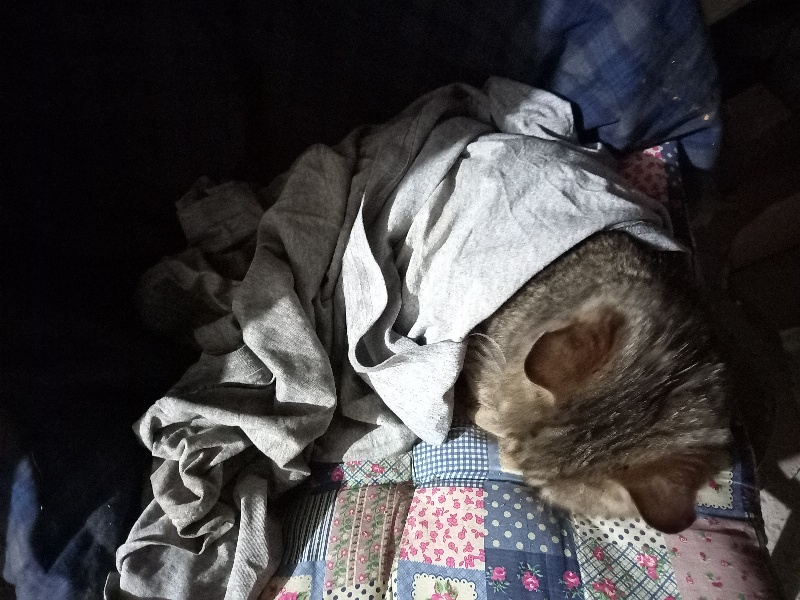
\includegraphics[width=\linewidth]{Slike/original.jpg}
        \caption{Originalna slika koja je skalirana}\label{sl_orig}
    \endminipage\hfill
    \minipage{0.32\textwidth}
        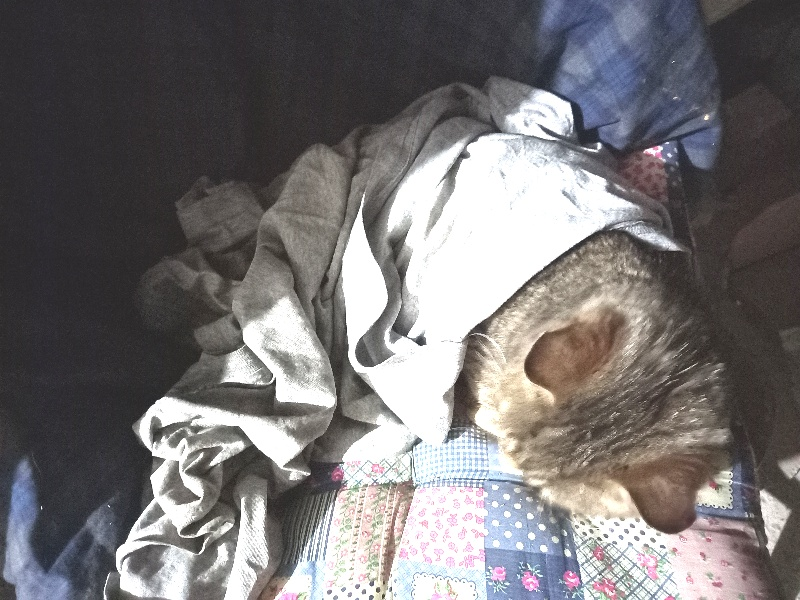
\includegraphics[width=\linewidth]{Slike/linearna.jpg}
        \caption{Slika nakon linearne transformacije}\label{sl_lin}
    \endminipage\hfill
    \minipage{0.32\textwidth}%
        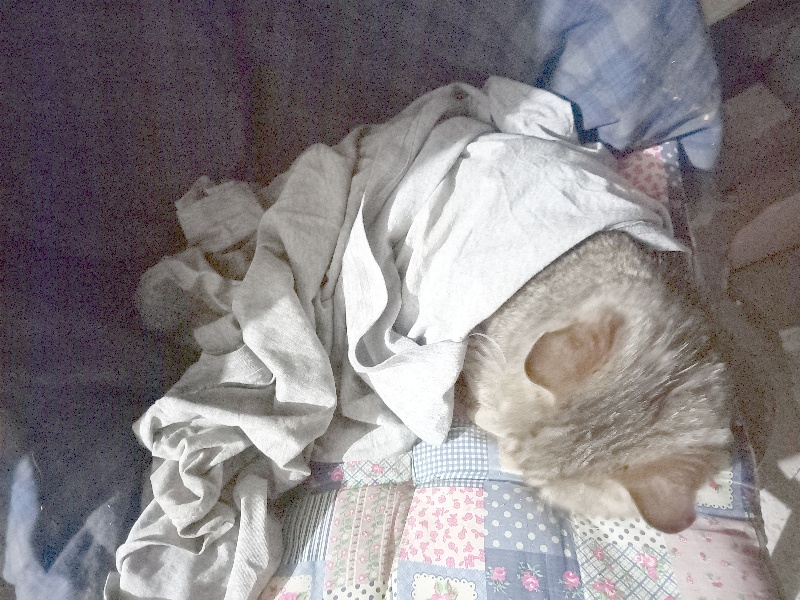
\includegraphics[width=\linewidth]{Slike/gama.jpg}
        \caption{Slika nakon gama transformacije}\label{sl_gama}
    \endminipage
\end{figure}

Gama korekcija bi trebala da daje manji efekat zasićenosti jer je mapiranje nelinearno i ne postoji numerička zasićenost kao u linearnoj metodi (ukoliko vrijednost padne ispod 0, zaokružuje se na 0, a ukoliko pređe 255 zaokružuje se na 255 u linearnoj metodi). Možemo više uporediti ove tri slike ukoliko im isplotamo histograme, što će biti pokazano u sljedećem dijelu tutorijala.

\subsection*{Histogrami slika}

Histogrami su skupljeni brojevi podataka koji su organizirani u set predefiniranih \textit{binova}. U slučaju histograma slika, u ovom tutorijalu govorimo o broju različitih intenziteta piksela na jednoj slici, ali možemo tražiti histogram bilo čega što nas zanima na slici, ne samo intenziteta piksela. 

U sljedećem primjeru ćemo izračunati histograme prethodne tri slike \ref{sl_orig}, \ref{sl_lin} i \ref{sl_gama}. 

\begin{lstlisting}
#include <opencv4/opencv2/highgui.hpp>
#include <opencv4/opencv2/core.hpp>
#include <opencv4/opencv2/imgproc.hpp>
#include <opencv4/opencv2/imgcodecs.hpp>
#include <opencv4/opencv2/core/fast_math.hpp>
#include <vector>

int main() {

    // Ucitavanje slike kojoj trazimo histogram:
    cv::Mat slika = cv::imread("../original.jpg", cv::IMREAD_COLOR);

    // Razdvajanje slike na 3 kanala (B, G i R):
    std::vector<cv::Mat> kanali;
    cv::split(slika, kanali);

    // Kako radimo sa B, G i R prostorima, znamo da su njihove vrijednosti od 0 do 255:
    int histSize = 256;
    float range[] = {0, 256};
    const float* histRange[] = {range};

    cv::Mat b_hist, g_hist, r_hist;

    // Postoji funkcija u OpenCV-u koja nam racuna histogram:
    cv::calcHist(&kanali[0], 1, 0, cv::Mat(), b_hist, 1, &histSize, histRange, true, false);
    cv::calcHist(&kanali[1], 1, 0, cv::Mat(), g_hist, 1, &histSize, histRange, true, false);
    cv::calcHist(&kanali[2], 1, 0, cv::Mat(), r_hist, 1, &histSize, histRange, true, false);

    // Treba napraviti sliku koja ce prikazati histograme za B, G i R:
    int hist_sirina = 512, hist_visina = 400;
    int bin_sirina = cvRound((double) hist_sirina / histSize );
    cv::Mat histogramSlike(hist_visina, hist_sirina, CV_8UC3, cv::Scalar(0, 0, 0));

    // Prije iscrtavanja histograma, potrebno je normalizirati svaki histogram tako da vrijednosti
    // upadaju u opseg parametara koje smo naveli:
    cv::normalize(b_hist, b_hist, 0, histogramSlike.rows, cv::NORM_MINMAX, -1, cv::Mat());
    cv::normalize(g_hist, g_hist, 0, histogramSlike.rows, cv::NORM_MINMAX, -1, cv::Mat());
    cv::normalize(r_hist, r_hist, 0, histogramSlike.rows, cv::NORM_MINMAX, -1, cv::Mat());

    // Crtanje histograma tako sto pristupamo binovima i crtamo vrijednosti:
    for(int i = 1; i < histSize; i++) {
        cv::line(histogramSlike, cv::Point(bin_sirina * (i - 1), hist_visina - cvRound(b_hist.at<float>(i - 1))),
                 cv::Point(bin_sirina * (i), hist_visina - cvRound(b_hist.at<float>(i))), cv::Scalar(255, 0, 0), 2, 8, 0);
        cv::line(histogramSlike, cv::Point(bin_sirina * (i - 1), hist_visina - cvRound(g_hist.at<float>(i - 1))),
                 cv::Point(bin_sirina * (i), hist_visina - cvRound(g_hist.at<float>(i))), cv::Scalar(0, 255, 0), 2, 8, 0);
        cv::line(histogramSlike, cv::Point(bin_sirina * (i - 1), hist_visina - cvRound(r_hist.at<float>(i - 1))),
                 cv::Point(bin_sirina * (i), hist_visina - cvRound(r_hist.at<float>(i))), cv::Scalar(0, 0, 255), 2, 8, 0);
    }

    // Prikaz slike i histograma te slike:
    cv::imshow("Slika", slika);
    cv::imshow("Histogram", histogramSlike);

    cv::waitKey();

    return 0;
}
\end{lstlisting}

Kako bismo izračunali histogram slike koja je u BGR formatu učitana, bilo je potrebno prvo podijeliti na njena tri kanala korištenjem funkcije \lstinline{cv::split}. Postoji funkcija u OpenCV-u koja nam omogućuje računanje histograma \lstinline{cv::calcHist} kojoj smo proslijedili odgovarajuće parametre (naznačeno je u komentarima koda zašto se neke vrijednosti prosljeđuju). Bilo je onda potrebno napraviti novi objekat tipa \lstinline{cv::Mat} koji će zapravo biti slika koja je histogram - naznačili smo njenu veličinu, tip i boju kojom će svi pikseli biti inicijalizirani (crna). Nakon toga uz pomoć funkcije \lstinline{cv::normalize} normaliziriamo histogram svakog kanala tako da se može fino upisati u novonapravljeni objekat \lstinline{histogramSlike}. Ucrtavanje histograma radimo preko funkcije \lstinline{cv::line} koja nam crta linije tako što povezujemo vrijednost iz trenutnog elementa niza \lstinline{b_hist}, \lstinline{g_hist} i \lstinline{r_hist} sa prethodnim. Dobiveni histogrami slika \ref{sl_orig}, \ref{sl_lin} i \ref{sl_gama} su prikazani na slikama \ref{sl_hist_orig}, \ref{sl_hist_lin} i \ref{sl_hist_gama}, respektivno.


\begin{figure}[H]
    \minipage{0.32\textwidth}
        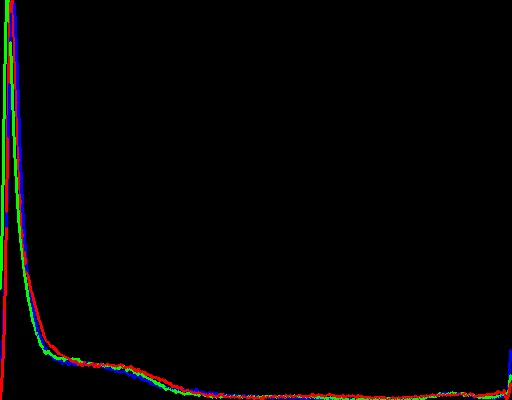
\includegraphics[width=\linewidth]{Slike/histogram_originala.jpg}
        \caption{Histogram originalne slike}\label{sl_hist_orig}
    \endminipage\hfill
    \minipage{0.32\textwidth}
        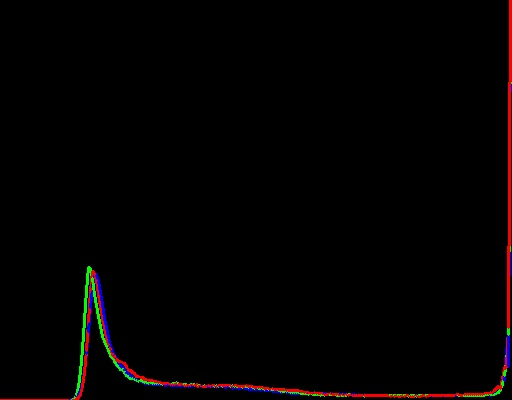
\includegraphics[width=\linewidth]{Slike/histogram_linearne.jpg}
        \caption{Histogram slike nakon linearne transformacije}\label{sl_hist_lin}
    \endminipage\hfill
    \minipage{0.32\textwidth}%
        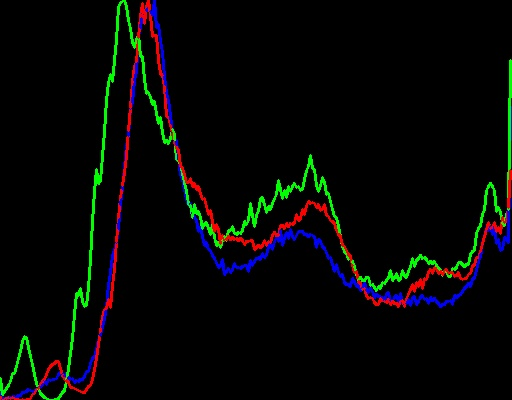
\includegraphics[width=\linewidth]{Slike/histogram_game.jpg}
        \caption{Histogram slike nakon gama transformacije}\label{sl_hist_gama}
    \endminipage
\end{figure}

Ono što možemo očitati je da kod originalne slike veliki dio vrijednosti piksela je u tamnom dijelu. Linearnom transformacijom smo postigli pomjeranje vrijednosti piksela više ka središnjem dijelu, ali opet vidimo da ima \textit{peak} prema tamnijem dijelu, iako nije toliko velik kao kod originala. Gama transformacijom smo uspjeli da vrijednosti piksela otprilike izjednačimo tako da više nisu u tamnijem dijelu (što smo i naveli da će se desiti prilikom gama transformacije).

\subsubsection*{Zadatak 1}

Uslikati (ili naći na internetu) sliku koja je previše svijetla. Uraditi linearnu i gama transformaciju nad njom, napraviti histograme slika i komentarisati rezultate koji su dobiveni.

\subsection*{Izjednačavanje histograma u OpenCV-u}

Izjednačavanje histograma predstavlja metodu koja popravlja kontrast slike, kako bi se razvukao opseg intenziteta. Kako bismo što bolje shvatili ovaj koncept, najbolje je da ga pokažemo na primjeru. 

\begin{lstlisting}
#include <opencv4/opencv2/highgui.hpp>
#include <opencv4/opencv2/core.hpp>
#include <opencv4/opencv2/imgproc.hpp>

int main() {

    // Ucitavanje slike:
    cv::Mat slika = cv::imread("../original.jpg", cv::IMREAD_COLOR);

    // Treba nam grayscale slika:
    cv::Mat grayscale;
    cv::cvtColor(slika, grayscale, cv::COLOR_BGR2GRAY);

    // Sad trebamo da izjednacimo histogram nad ovom slikom:
    cv::Mat izjednacena;
    cv::equalizeHist(grayscale, izjednacena);

    cv::imshow("Grayscale", grayscale);
    cv::imshow("Nakon izjednacenja histograma", izjednacena);

    cv::waitKey();

    return 0;
}
\end{lstlisting}

Prethodni kod pokazuje kako možemo uz pomoć OpenCV funkcije \lstinline{cv::equalizeHist} da izjednačimo histogram \textit{grayscale} slike. Ova funkcija prima dva parametra - originalnu sliku u \textit{grayscale}-u i izlaznu sliku u koju se stavlja rezultat izjednačenja histograma (oba parametra su tipa \lstinline{cv::Mat}).

Prethodni program smo izvršili nad istom slikom kao maloprije i dobili smo rezultat koji prikazan na slikama \ref{sl_gray} i \ref{sl_izj}.

\begin{figure}[H]
    \minipage{0.49\textwidth}
        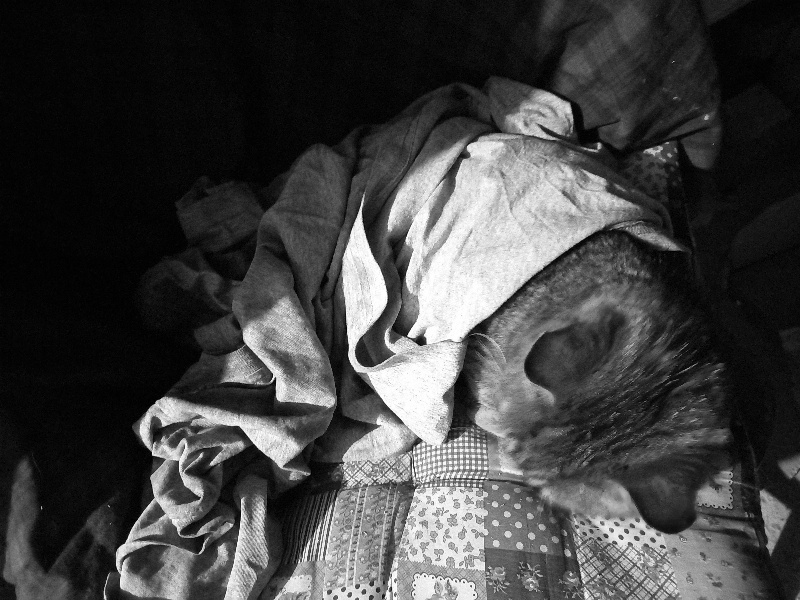
\includegraphics[width=\linewidth]{Slike/grayscale.jpg}
        \caption{Originalna \textit{grayscale} slika}\label{sl_gray}
    \endminipage\hfill
    \minipage{0.49\textwidth}
        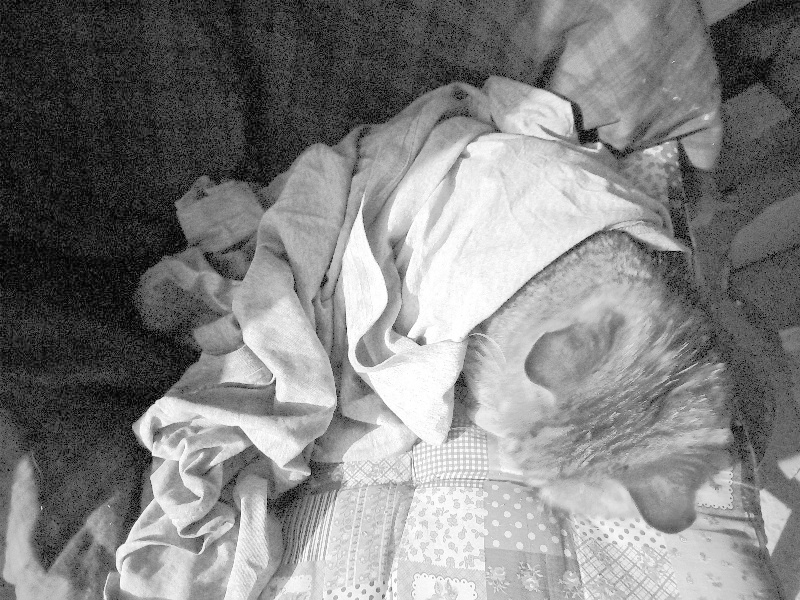
\includegraphics[width=\linewidth]{Slike/izjednacena.jpg}
        \caption{Slika nakon izjednačenja histograma}\label{sl_izj}
    \endminipage\hfill
\end{figure}

Ukoliko iskoristimo prethodni kod da izračunamo histograme ovih slika (bez da ih razbijamo na 3 kanala jer su obje grayscale), dobijamo histograme koji su prikazani na slikama \ref{sl_hist_gray} i \ref{sl_hist_izj}.

\begin{figure}[H]
    \minipage{0.49\textwidth}
        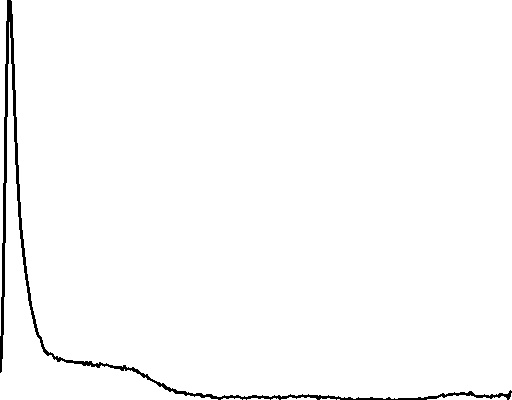
\includegraphics[width=\linewidth]{Slike/histogram_grayscale.jpg}
        \caption{Histogram originalne \textit{grayscale} slike}\label{sl_hist_gray}
    \endminipage\hfill
    \minipage{0.49\textwidth}
        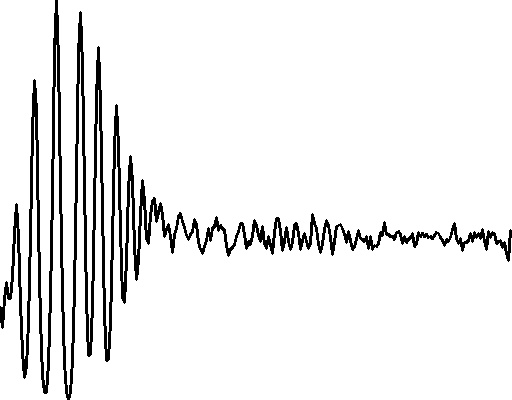
\includegraphics[width=\linewidth]{Slike/histogram_izjednacene.jpg}
        \caption{Histogram slike nakon izjednačenja histograma}\label{sl_hist_izj}
    \endminipage\hfill
\end{figure}


\subsubsection*{Zadatak 2}

Komentarisati dobivene histograme iz prethodnog primjera. Šta smo dobili?

\subsection*{Napomene}

Korištena tema za prikaz C++ koda na tutorijalima je \href{https://ethanschoonover.com/solarized/}{\lstinline{solarized}}\cite{solarized}.

\printbibliography


\end{document}
